\subsubsection{Model conceptual}
Per poder provar la configuració que fem de Hibernate i executar un petit programa que persisteixi un parell d'objectes, implementem dues classes del model conceptual del domini. No obstant, cal veure que les classes són simples, donat que la única relació que contenen és la que comparteixen. No modelem, doncs, cap altre relació ni cap comportament, donat que no ho necessitem per a provar Hibernate.

\begin{figure}[h]
	\centering
	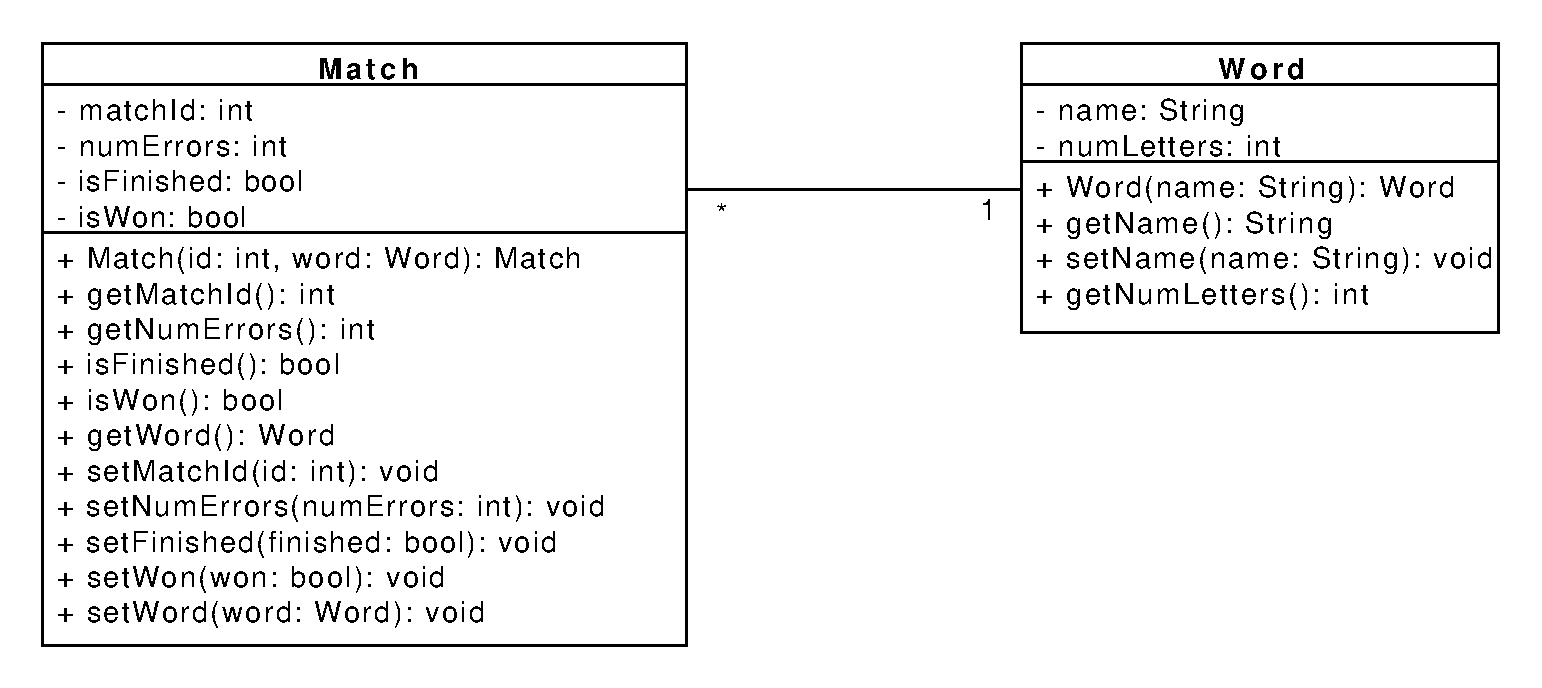
\includegraphics[width=0.8\linewidth]{figures/concept_model_impl.pdf}
	\caption{Diagrama del model conceptual implementat}
	\label{fig:conceptmodel}
\end{figure}

Tal i com podem veure a la figura \ref{fig:conceptmodel}, implementem la classe Partida (Match) i Paraula (Word), amb els seus atributs simples i la relació entre elles. Ja podem procedir a configurar Hibernate.

\subsubsection{Configurant Hibernate}
En primer lloc, caldrà que el projecte de Java que hem creat contingui les llibreries necessàries que composen el paquet de Hibernate. Aquestes inclusions les fem mitjançant l'eina Maven, com ja hem explicat abans. Concretament, hem d'afegir un driver JDBC de connexió per la base de dades concreta que estem fent servir, a més del nucli del propi framework i una llibreria externa (\texttt{javassist}) que és necessària per donar suport a la \emph{reflexió estructural}, de la qual Hibernate fa ús.

Per tal que Hibernate persisteixi el model del nostre domini, cal que li proporcionem una mínima configuració. Fonamentalment, ens cal donar-li l'adreça a la qual ha de fer la connexió amb la base de dades relacional, l'usuari i la contrasenya amb els quals ens connectarem i l'esquema contra el qual voldrem executar el nostre sistema. Tot això s'indica al fitxer \texttt{hibernate.cfg.xml}. També configurem en aquest fitxer algunes propietats que necessitem perquè funcioni correctament o perquè ens poden resultar útils. La configuració que apliquem finalment a Hibernate és la següent:

\begin{minted}{xml}
<hibernate-configuration>
    <session-factory name="HibernateUtil">
        <!-- Connection parameters -->
        <property name="hibernate.connection.driver_class">
            org.postgresql.Driver
        </property>
        <property name="hibernate.connection.url">
            jdbc:postgresql://localhost:5432/asdb
        </property>
        <property name="hibernate.connection.username">postgres</property>
        <property name="hibernate.connection.password">postgres</property>
        <!-- Hibernate properties -->
        <property name="hibernate.default_schema">public</property>
        <property name="hibernate.dialect">
            org.hibernate.dialect.PostgreSQLDialect
        </property>
        <property name="hibernate.show_sql">true</property>
        <property name="hibernate.hbm2ddl.auto">update</property>
    </session-factory>
</hibernate-configuration>
\end{minted}

\begin{itemize}
	\item \textbf{\texttt{default\_schema}:} és el nom de l'esquema que atacarà Hibernate, a la base de dades \texttt{asdb}. El valor és \texttt{public}, perquè és el que defineix per defecte PostgreSQL quan crea una base de dades.
	\item \textbf{\texttt{dialect}:} per tal que Hibernate pugui fer les associacions correctes segons els tipus de dades, cal indicar-li quin \emph{dialecte} de SQL és l'emprat per la base de dades.
	\item \textbf{\texttt{show\_sql}:} ens permet habilitar l'enregistrament a la consola de les sentències SQL que genera Hibernate.
	\item \textbf{\texttt{hbm2ddl.auto}:} aquesta opció és necessària per poder modificar l'esquema de la base de dades quan s'executa el nostre sistema, de manera que si afegim una nova classe al model conceptual, Hibernate s'ocupa de crear la taula o taules necessàries per a reflectir els canvis. Cal notar que aquesta propietat pot ser perillosa si es deixa amb el valor \texttt{update} en un codi de producció, donat que es podria modificar sense voler o amb efectes colaterals l'esquema d'una base de dades en explotació. Per evitar-ho, també es poden aplicar altres valors, com ara \texttt{validate}, el qual només valida l'esquema, però no el modifica.
\end{itemize}

\subsubsection{Anotant les classes}
Tal i com hem dit, per aquesta pràctica farem servir el model d'anotacions que ens ofereix JPA (\emph{Java Persistence API}) i que Hibernate suporta. Tot seguit mostrem com queden anotades les classes \texttt{Match} i \texttt{Word}, amb els seus membres corresponents:

\begin{minted}{java}
    @Entity
    @Table(name=Word.TABLE)
    public class Word implements Serializable {
        public static final String TABLE = "word";
        
        @Id @Column
        private String name;
        
        @Column
        private int numLetters;
        ...
    }
    
    @Entity
    @Table(name=Match.TABLE)
    public class Match implements Serializable {
    
        public static final String TABLE = "match";
    	
        @Id @Column
        private int matchId;
    	
        @Column
        private int numErrors;
    	
        @Column
        private boolean isFinished;
    	
        @Column
        private boolean isWon;
    	
        @ManyToOne
        private Word word;
        ...
    }
\end{minted}

Ara cal indicar al fitxer de configuració de Hibernate quines són les classes del model conceptual del nostre domini de les quals volem en gestioni la persistència. Per fer-ho, simplement ens cal afegir, per cadascuna, un element de tipus \texttt{mapping} a l'element \texttt{session-factory} que ja tenim definit al fitxer:

\begin{minted}{xml}
    <mapping class="edu.upc.fib.wordguess.domain.model.Match"/>
    <mapping class="edu.upc.fib.wordguess.domain.model.Word"/>
\end{minted}

\subsubsection{Provant Hibernate}
Implementem tot seguit un petit programa de prova per inserir un objecte de la classe \texttt{Match}, que té una relació amb un objecte \texttt{Word}. El codi del programa el trobem al fitxer \texttt{TestApp.java} i és força senzill:

\begin{minted}{java}
    public static void main( String[] args ) {
        Session session = HibernateUtil.getSessionFactory().openSession();
        session.beginTransaction();
        
        Word word = new Word("giraffe");
        Match match = new Match(1, word);
        
        session.save(word);
        session.save(match);
        
        session.getTransaction().commit();
        session.close();
        HibernateUtil.shutdown();
    }
\end{minted}

Un cop executem aquest codi, podem esbrinar fàcilment quin ha estat l'efecte obrint una connexió amb la base de dades. Per fer-ho, podem TODO!!!!!
